\chapter{Introduction}
\label{intro}
%Chebfun is a Matlab package that allows for computation of functions via Chebyshev polynomial approximations. It was developed at Oxford's Numerical Analysis Group by Zachary Battles under the supervision of Nick Trefethen in 2006 \cite{battles2004extension}. It has since been extensively updated to include adaptive piecewise-approximations \cite{pachon2010piecewise}, as well as solve ordinary differential equations and boundary value problems \cite{driscoll2008chebop,birkisson2012automatic,birkisson2013numerical}.

A distinctive and powerful mode of scientific computation has emerged recently in which mathematical functions are represented by high-accuracy numerical analogs, which are then manipulated or analyzed numerically using a high-level toolset~\cite{Trefethen2015}. The most prominent example of this style of computing is the open-source Chebfun project~\cite{battles2004extension,Driscoll2014}. Chebfun, which is written in MATLAB, samples a given piecewise-smooth univariate function at scaled Chebyshev nodes and automatically determines a Chebyshev polynomial interpolant for the data, resulting in an approximation that is typically within a small multiple of double precision of the original function. This approximation can then be operated on and analyzed with algorithms that are fast in both the asymptotic and real-time senses. Notable operations include rootfinding, integration, optimization, solution of initial- and boundary-value problems, eigenvalues of differential and integral operators, and solution of time-dependent PDEs.

The main aim of Chebfun is to allow for computation that feels symbolic, but is computed numerically in a way that is both fast and accurate to machine precision similar to what floating-point arithmetic achieves for numbers \cite{trefethen2015computing}. Chebfun uses Chebyshev polynomial interpolants because they are highly accurate, and stable even for large amounts of points \cite{mason2002chebyshev,Trefethen2013}.  In particular if we have a Chebyshev interpolant $p_n(x)$ of a analytic function $f(x)$ then the Chebyshev interpolant are spectrally accurate, as stated in Theorem 6 \cite{trefethen2000spectral}:
\begin{thm} Suppose $f(z)$ is analytic on and inside the Bernstein ellipse $E_\rho$. Let $p_n$ be the polynomial that interpolates $f(z)$ at $n+1$ Chebyshev points of the second kind. Then there exists a constant $C>0$ such that for all $n>0$,
	$$ \left \| f(x)-p_n(x) \right \|_{\infty} \leq C  \rho^{-n}.$$
\end{thm}
If $f(x)$ is Lipschitz continuous on $[-1,1]$ then
\begin{equation}
f(x) = \sum_{k=0}^\infty a_k T_k(x), \quad a_k = \frac{2}{\pi} \int_{-1}^1 \frac{f(x) T_k(x)}{\sqrt{1-x^2}} dx,
\end{equation}
where $T_k$ denotes the degree $k$ Chebyshev polynomial (and for $a_0$, we multiply by $\frac{1}{\pi}$ instead of $\frac{2}{\pi}$). Furthermore if $p_n(x)$ is the $n$th degree Chebyshev interpolant then
\begin{equation}
f(x)-p_n(x) = \sum_{k=n+1}^{\infty} a_k \lp T_k(x)-T_m(x)\rp,
\end{equation}
where
\begin{equation}
m = \left [ (k+n-1)(\text{mod }2n) - (n-1)\right ],
\end{equation}
implying we can determine the accuracy of the interpolant $p_n(x)$ by inspecting the Chebyshev coefficients \cite{Trefethen2013}. Chebfun's {\tt standardChop} method determines the minimum required degree by searching for a plateau of low magnitude coefficients \cite{Aurentz:2017:CCS:3034774.2998442}.  For example, Figure~\ref{Coeff_example} shows the first 128 coefficients of $f(x)=\exp \lp \sin \lp \pi x \rp \rp$. We see that all coefficients after the first 46 have magnitude less than $10^{-15}$. In this case, Chebfun determines the ideal degree to be 50.
\begin{figure}
	\centering
	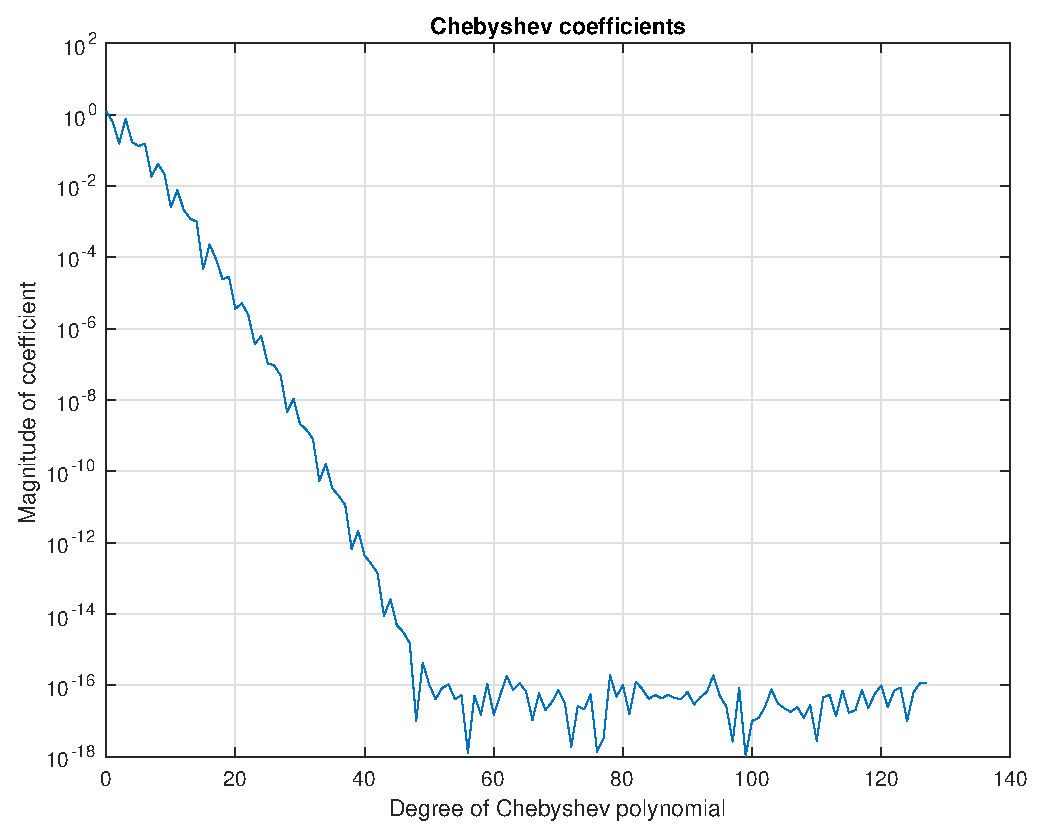
\includegraphics[scale = 0.5]{Chapter1/coeff_plot.eps}
	\caption{Chebyshev coefficients for $f(x)=\exp \lp \sin \lp \pi x \rp \rp$.}
	\label{Coeff_example}
\end{figure}

Townsend and Trefethen extended the 1D Chebfun algorithms to 2D functions over rectangles in Chebfun2~\cite{townsend2013extension,Townsend2014}, which uses low-rank approximations in an adaptive cross approximation. The construction and manipulation of 2D approximations is suitably fast for a wide range of smooth examples. Most recently, Hashemi and Trefethen created an extension of Chebfun called Chebfun3 for 3D approximations on hyperrectangles using low-rank ``slice--Tucker'' decompositions~\cite{Hashemi2017}. The range of functions that Chebfun3 can cope with in a reasonable interactive computing time is somewhat narrower than for Chebfun2, as one would expect. 

An alternative to Chebfun and related projects ported to other languages is sparse grid interpolation. Here one uses linear or polynomial interpolants on hierarchical Smolyak grids. Notable examples of software based on this technique are the Sparse Grid Interpolation Toolbox~\cite{Klimke2005} and the Sparse Grids Matlab Kit~\cite{Back2011}. An advantage of these packages is that they are capable of at least medium-dimensional representations on hyperrectangles. However, they seem to be less focused on high-accuracy approximation for a wide range of functions, and they are less fully featured than the Chebfun family. These methods are also highly nonisotropic.

The more general problem of approximation of a function with high pointwise accuracy over a nonrectangular domain $\Omega \subset \R^d$ allows more limited global options than in the hyperrectangular case. Neither low-rank nor sparse grid approximations have any clear global generalizations to this case. Two techniques that can achieve spectral convergence for at least some such domains are radial basis functions~\cite{Fornberg2015} and Fourier extension or continuation~\cite{adcock2014resolution}, but neither has been conclusively demonstrated to operate with high speed and reliability over a large collection of domains and functions.

In this dissertation, we expand on the ideas of Chebfun to create approximations that are both accurate and infinitely smooth via partition of unity, a set of functions whose sum must add to one. Partition of unity schemes have been widely used for interpolation \cite{franke1980smooth,mclain1976two,shepard1968two} and solving PDEs \cite{griebel2000particle,safdari2015radial}. Suppose we have an overlapping covering $\{ \Omega_k \}_{k=1}^N$ on a bounded region $\Omega$. A partition of unity is a collection of real valued functions $\{w_k(\vect{x)}\}_{k=1}^N$ such that:

\begin{itemize}
	\item $w_k(\vect{x})$ has support within $\Omega_k$,
	\item each $w_k(\vect{x})$ is nonnegative,
	\item $\forall x \in \Omega, \quad \sum_{k=1}^N w_k(\vect{x})=1$.
\end{itemize}
The functions $\{w_k(\vect{x})\}_{k=1}^N$ are called the \textit{weights} of the partition. We can use the partition of unity $\{w_k(\vect{x})\}_{k=1}^N$ to construct an approximating function. Suppose that for $m \geq 0$ we have a function $f \in C^{m}(\Omega)$, each weight $w_k(\vect{x})\in C^{m}(\Omega)$ and for each patch $\Omega_k$ we have an approximation $s_k(\vect{x})$ of $f(\vect{x})$. Then the function
\begin{equation}
\label{POUAPPROX}
s(\vect{x}) = \sum_{k=1}^N w_k(\vect{x})s_k(\vect{x})
\end{equation}
can be used to approximate $f(\vect{x})$ and its derivatives \cite{wendland2004scattered}.

\begin{thm}
	\label{PUMCON}
	Suppose $f \in C^{m}(\Omega)$ and for each patch $\Omega_k$ we have a function $s_k(\vect{x})$ such that
	$$ \|D^{\alpha}f(\vect{x})-D^{\alpha} s_k(\vect{x})\|_{L_{\infty}(\Omega_k)} \leq \varepsilon_k(\alpha),\quad \vect{x} \in \Omega $$
	for all $|\alpha| \leq k$. Thus for $j\leq m$, if $s(x)$ is the approximation (\ref{POUAPPROX}) then
	\begin{equation}
	\left \| D^{\alpha}f(\vect{x})-D^{\alpha} s_k(\vect{x}) \right \|_{L_{\infty}(\Omega_k)} \leq \sum_{k=1}^N\sum_{\beta \leq \alpha} \binom{\alpha}{\beta} \left \| D^{\alpha-\beta} w_k(\vect{x}) \right \|_{L_{\infty}(\Omega_k)} \epsilon_k(\alpha).
	\end{equation}
\end{thm}
\begin{proof}
	Since $\sum_{k=1} w_k(\vect{x})=1$, $\sum_{k=1} w_k(\vect{x})f(\vect{x})=f(\vect{x})$. Thus
	\begin{equation}
	\begin{aligned}
	D^{\alpha}f(\vect{x})-D^{\alpha} s_k(\vect{x}) &= D^{\alpha} \sum_{k=1}^N w_k(\vect{x})(f(\vect{x})-s_k(\vect{x}x)) \\
	&= \sum_{k=1}^N\sum_{\beta \leq \alpha} \binom{\alpha}{\beta} D^{\alpha-\beta} w_k(\vect{x}) \lp D^{\beta} f(\vect{x})-s_k^{(i)}(\vect{x}) \rp.
	\end{aligned}
	\end{equation}
	The result follows from here by the triangle inequality.
\end{proof}

A major goal of Chebfun has been to develop methods to automatically find solutions to ODES using Chebyshev approximations \cite{driscoll2008chebop,birkisson2012automatic,birkisson2013numerical}. We build on our overlapping domain approximations to solve boundary-value and evolutionary PDEs efficiently via domain decomposition methods. Overlapping domain decomposition has been recognized as a valuable aid in solving partial differential equations since Schwarz first described his alternating method in 1870. (For straightforward introductions to the topic, see~\cite{Dolean2015,Smith2004}; for a more historical perspective, see~\cite{Gander2008}.) Overlapping decomposition provides a way to solve a problem on a global domain by exploiting its reduction to smaller subdomains. This creates geometric flexibility and allows special effort to be focused on small parts of the domain when appropriate. Domain decomposition also has a natural parallelism that is particularly attractive in the increasingly multicore context of scientific computing.

For a linear PDE, one typically seeks to apply a preconditioner for a Krylov iteration such as GMRES, in the form of solving problems on overlapping subdomains whose boundary data is in part determined by values of the solution in other subdomains. In the parallel context this is achieved by an additive Schwarz (AS) scheme. When one partitions the unknowns of a global discretization into overlapping subsets, the best form of AS are restricted AS (RAS) methods~\cite{Cai1999}, which do not allow multiple domains to update shared unknowns independently and thus over-correct. Typically, then, the subdomain problems are solved on overlapping sets, but the results are distributed in a nonoverlapping fashion. 
%

Cai and Keyes~\cite{Cai2002} proposed instead modifying the \emph{nonlinear} problem using the Schwarz ansatz. In addition to yielding a preconditioned linearization for the Krylov solver, the preconditioned nonlinear problem exhibited more robust convergence for the Newton iteration than did the original nonlinear problem. They called their method ASPIN, short for \textit{additive Schwarz preconditioned inexact Newton}. Subsequently, Dolean et al.~\cite{Dolean2016} pointed out that Cai and Keyes did not use the RAS form of AS preconditioning, and they proposed an improved variant called RASPEN that does. % We refer to this type of nonlinear preconditioning as \emph{Schwarz--Newton--Krylov} (SNK), because the Schwarz ansatz is applied before the linearization begins.

A major motivation for our focus on domain decomposition methods is for the numerical solutions of a fourth order blinking eye model. In the past, on overset grid method has been used to solve models on a realistic eye shaped domain \cite{chesshire1990composite,henshaw1998ogen,li2012model,li2015computed}. The overset grid method discritizes the PDE by covering the domain with overlapping finite difference grids coupled together through interpolation. This method, while highly effective, is limited in accuracy. Driscoll and Braun developed a method to simulate parabolic flow on a blinking eye shaped domain, which was discretized using a tensor product Chebyshev polynomial approximation \cite{driscoll2018simulation}. While the use of a spectral approximation led to higher accuracy, tensor product polynomials are expensive to use computationally since the matrices representing the PDE discritizations are dense.

 The outline of this dissertation is as follows. In Chapter~\ref{pu_1d}, we explore how we can recursively define partitions of unity in one dimension as well as examine how these approximations can be used to solve BVPs. We then generalize in Chapter~\ref{pu_nd} to an automatic way of creating multidimensional Chebyshev approximations on hyper-rectangles. The method also was then extends to arbitrary domains, via a least squares technique. For Chapter~\ref{snk_chap} we use an overlapping partition of a rectangle to create a new nonlinear preconditioned method using the additive Schwarz technique. We lastly in Chapter~\ref{chap_eye} apply our new preconditioned techniques on a fourth order model that represents the tear film fluid within a moving eye shaped domain. Our method allows us to obtain the resolution needed for higher accuracy.

